
\chapter{Analysis}

% bring up features from #Background
% features:

\section{Experiment Setup}

Each device in the testbed has at least three active Ethernet links:
One connecting it to a management server, and two connected to the
corresponding \Ac{dut} or \Ac{loadgen}. The management server (kaunas)
uses \Ac{pos} \cite{GallScho18} to set boot images, boot, run setup
and testing scripts on the testbed devices and collect script output
and artifact files containing test results.

As Figure \ref{setup} shows, each test contains two devices. The
\Ac{dut}, running \Ac{vpp}, and the \Ac{loadgen}, running MoonGen,
generating packets and sending them to the \Ac{dut} to test \Ac{vpp}.
\Ac{vpp} then forwards the packets back to the \Ac{loadgen} which
allows the \Ac{loadgen} to create accurate throughput and latency
measurements.
On the \Ac{dut} some debug information like error counts are being
gathered from the \Ac{vpp} CLI interface and Linux perf tools
\cite{perf} attach to the \Ac{vpp} process to collect time spent per
symbol and stats like CPU cycles or cache misses.

\begin{figure}[!ht]
\noindent\hspace{0.5mm}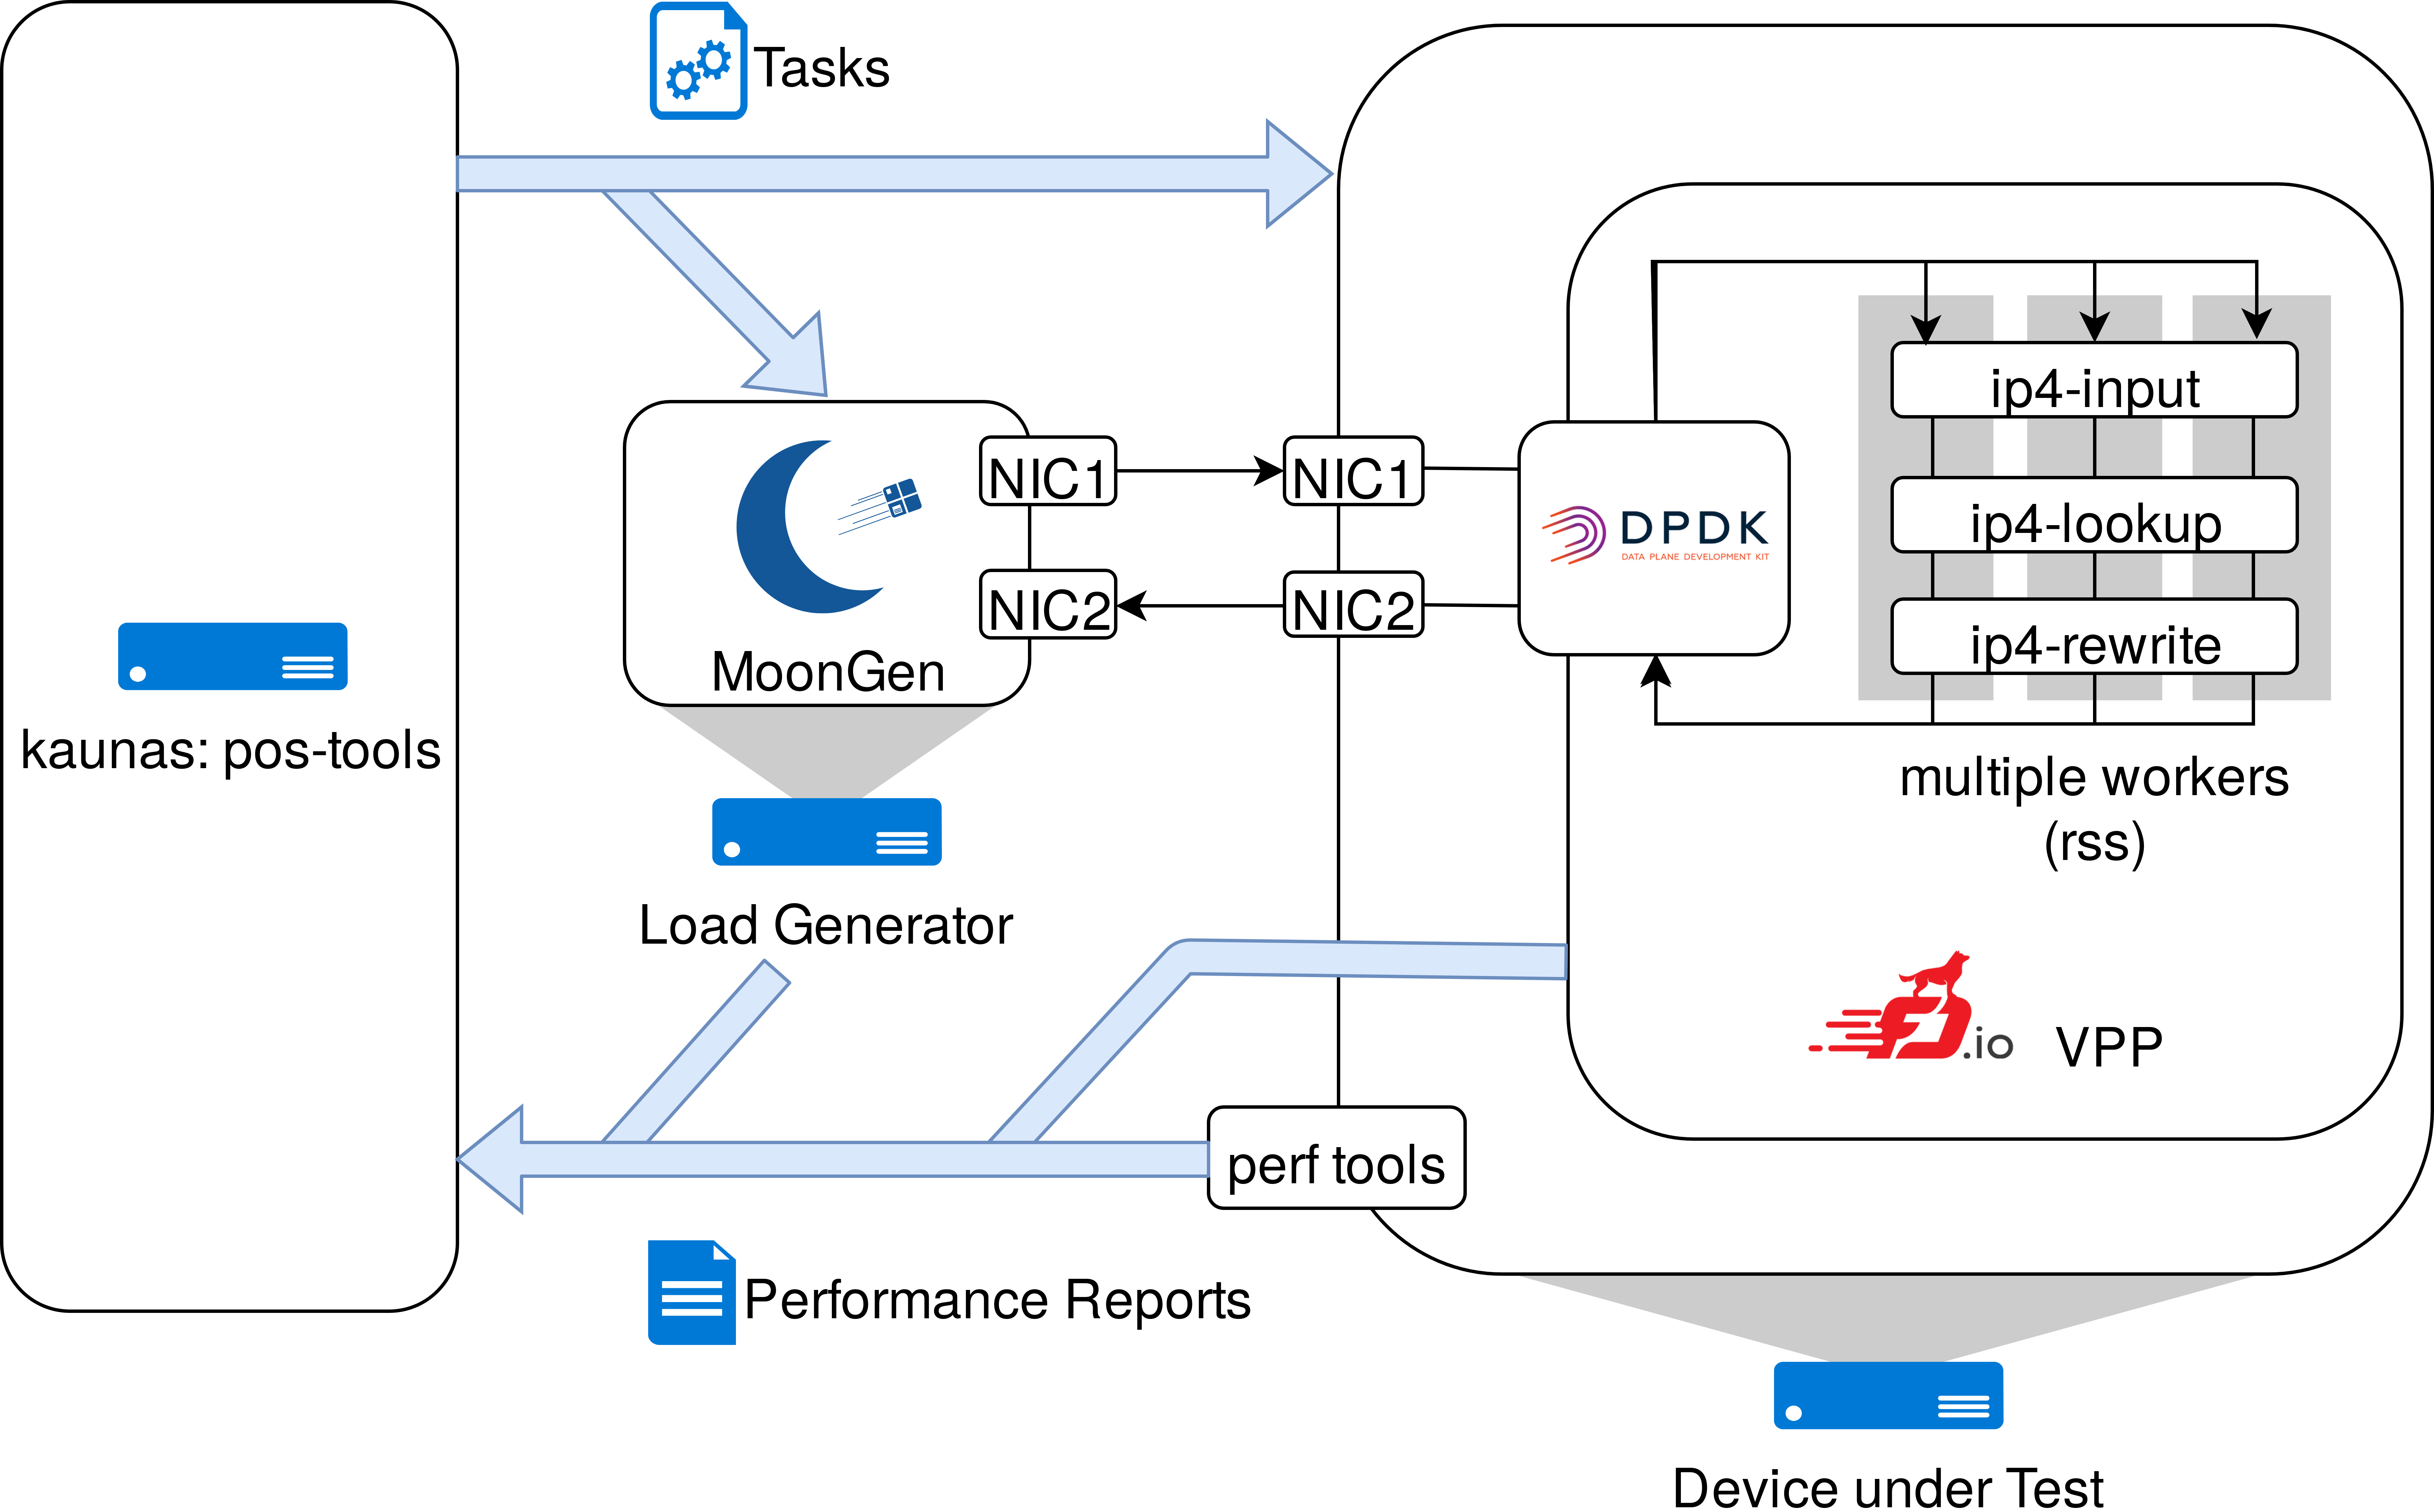
\includegraphics[width=\linewidth]{pics/topology.png}
\caption{Experiment setup for testing VPP with "kaunas" management server, \Ac{loadgen} and DUT}
\label{setup}
\end{figure}


\section{Possible Bottlenecks}

\subsection{Physical Link Speed}
\label{sec:linkspeed}

% - in many cases: 
% 	- 10GbE

Running \Ac{vpp} with only one worker, the physical link speed is never
the limiting factor. Usually this is 10GbE in this paper. Only with
multiple worker scenarios the 10Gb/s mark is quickly reached. A simple
way to address this is by testing with bidirectional traffic - sending
load to both of DUT's NICs and expecting VPP to forward it to both
NICs again. This way, the load on a single CPU core to be tested can
be doubled, without actually requiring faster links. Other options are
to reduce CPU clock speed or increase the CPU load artificially on a
per-packet basis, in order to create another, even more limiting
bottleneck on the CPU. The obvious solution, using a 40GbE link with
more bandwidth, was used for this paper.


\subsection{\Ac{loadgen} Speed}

% - loadgen speed
% 	- can saturate a 10GbE link with minimum sized ethernet frames for all tests conducted (14.88mpps)

Another limiting factor could be the load generator's speed of
generating load. MoonGen, the \Ac{loadgen} used for this paper, can
saturate a 10GbE link with minimum sized Ethernet frames for all tests
conducted. For a simple unidirectional 10GbE link this results in
14.88 Mpps \cite{emmerich2015assessing}.

% TODO: remove this if not relevant to the paper: 
% TODO: move this to the "internal paragraph" section

\label{sec:40gbelimit}

Using faster 40GbE with Intel XL710 NICs showed a soft throughput
limit of about 22.81 Mpps (min. frame size, unidirectional, standard
deviation: 0.22). This was observed with an Intel E5-2620 v3
(2.40GHz). This limit varies when increasing the frame size. Previous
work showed that the cause for this are bottlenecks inside the NIC.
\cite{emmerich2015moongen}

% TODO move this to link speed subsection

\subsection{Internal Bandwidth}

% pci bandwidth

Inside the DUT there is first of all the PCI bandwidth. All tested
NICs are connected by a PCIe 2.0 x8 link with a maximum transfer rate
of 32Gbit/s per direction. In theory a 40GbE link could exceed this
transfer rate. Because the tests in this paper are only done with
small packet sizes, the maximum reached packet generation rate of
around 22.8 Mpps results in significantly less than 32Gbit/s. For
bigger frame sizes, the width of PCI interfaces will have to be
increased, because otherwise it will become a bottleneck for
40GbE links.

% ram bandwidth

Secondly the Ethernet frames have to be moved to the main memory. It
typically supports between 1333 MT/s (the 10GbE system) or 2133 MT/s
(40GbE system) transmitting 64bit per message. This results in a
transfer rate of 85 GBit/s and 136 GBit/s. This should be sufficient
for 10GbE networking, 40GbE links require at least 2133MT/s memory.

\subsection{CPU Time per Packet}

As Section \ref{sec:cpubottleneck} will show, the CPU time spent per
packet is the biggest bottleneck. The following subsections describe
how this issue is dealt with in VPP.


% TODO:
% - vpp's cpu cycles: branch prediction, cycles/packet
% - memory latency: latency increases cpu time, caches can improve latency


\section{NICs with DPDK and VPP}

For VPP to utilize NICs up to their specified line rate, it relies on
\Ac{dpdk}. This introduces a few noteworthy optimizations:

\paragraph{RSS (Receive Side Scaling)}
\label{sec:rss}

When the NIC receives a packet, it can be configured to hash over
specified packet header fields to assign the packet to a receiving
queue. The idea is, to efficiently separate for example different IP
traffic flows early which can then be processed by several VPP workers
concurrently and independently. \cite{linguaglossa2017high}

\paragraph{Zero-Copy}

Because memory bandwidth is actually limited, it is important not to
move frames around unnecessarily. Therefore the NIC copies the
received frames to memory shared with VPP which is their final fixed
location. \cite{linguaglossa2017high}

\paragraph{Busy Polling}

Newer VPP versions have options to be either notified about new
packets in the shared memory via interrupts, or alternatively and
better suited for high performance applications, \Ac{vpp} workers can
be busy polling. The latter option reduces performance dependencies on
the hardware and kernel. \cite{vppdocs:rxmodes}

% TODO (no. this is already explained in the model)
% vpp's multithreading model: hqos, worker, main thread
% placement

\section{Packet Processing Graph}

\begin{figure}[!ht]
\noindent\hspace{0.5mm}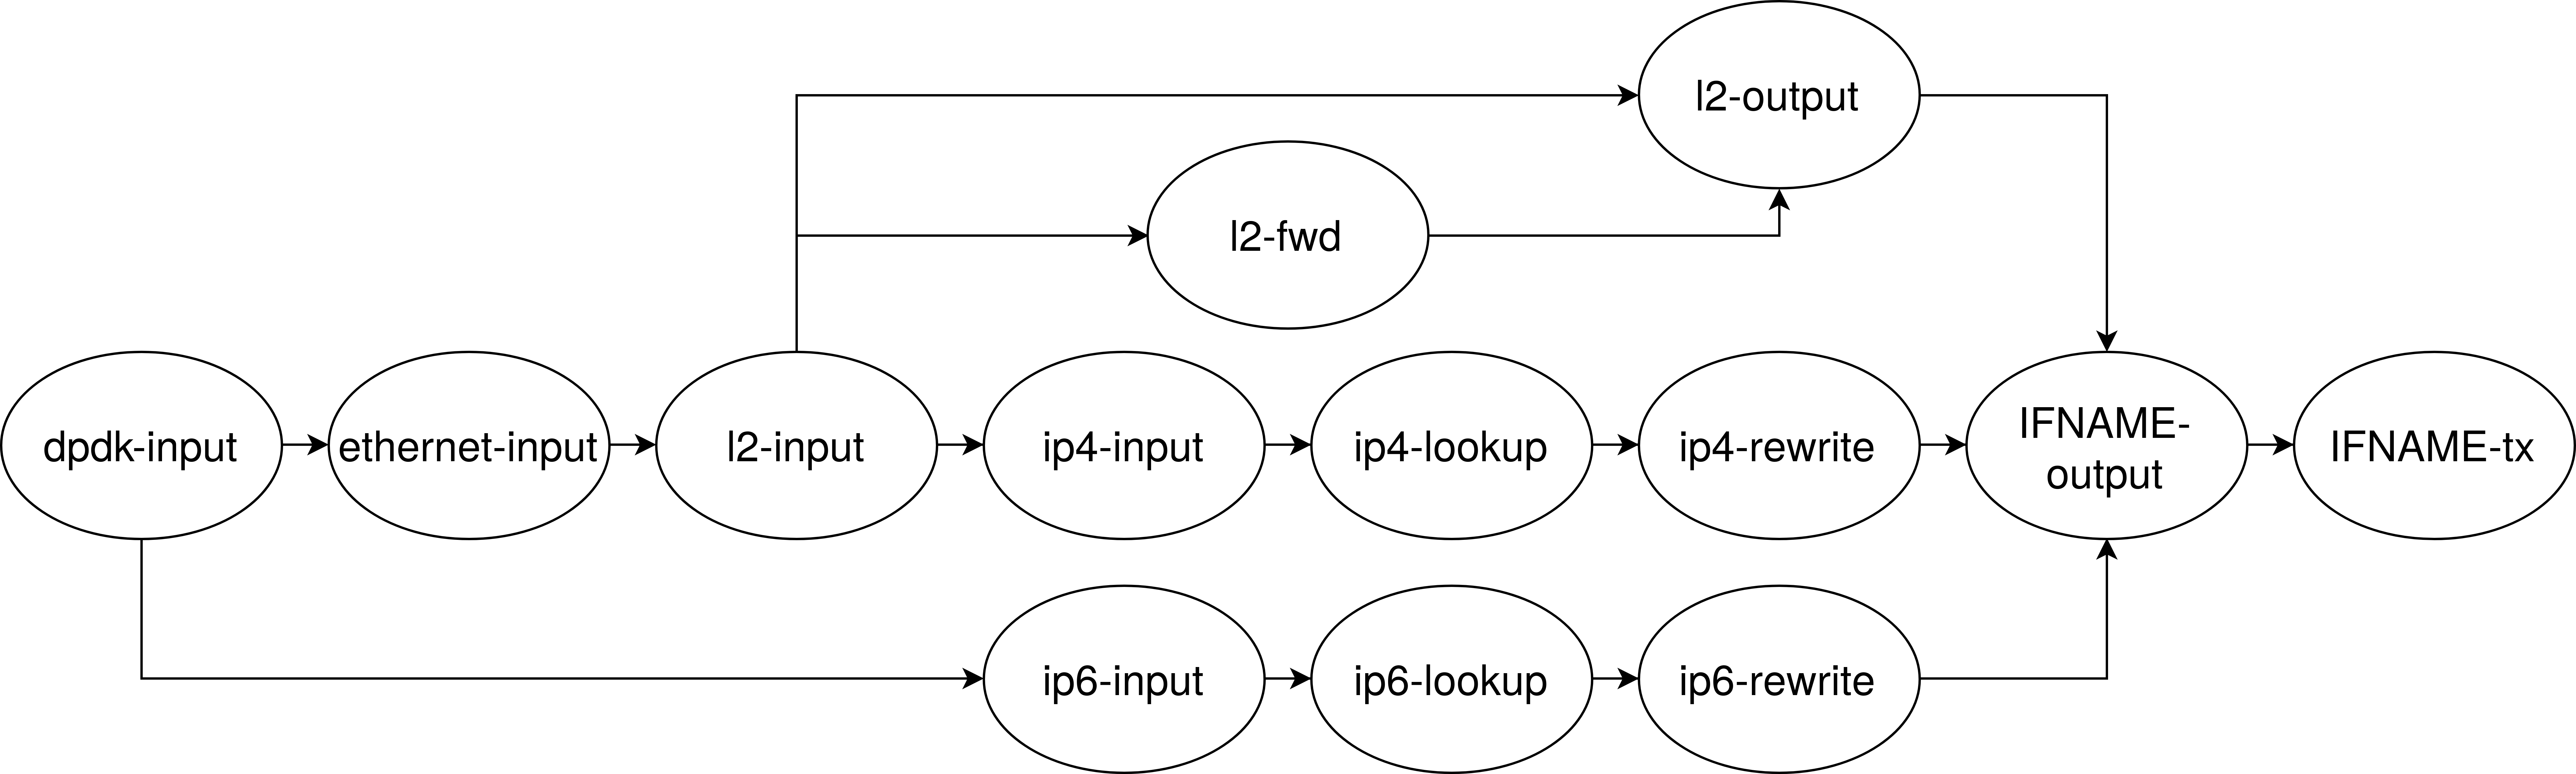
\includegraphics[width=\linewidth]{pics/vpp-nodes-horizontal.png}
\caption{VPP packet processing graph for xconnect, bridging, \Ac{ip4} routing and \Ac{ip6} routing. Other paths are left out. }
\label{nodegraph}
\end{figure}

% - modularity, feature rich
%	- visualize the parsing done in the first step as in the vpp paper and explain 
% 		bridging only: ip header parsing slowdown behaviour

VPP's packet processing is defined by the packet processing graph.
Figure \ref{nodegraph} illustrates selected packet paths important for
this paper. Depending on the plugins and configuration in place, this
graph can be customized for example to replace specific software
functions with hardware accelerators. Depending on the initial packet
parsing which happens in the "dpdk-input" and "l2-input" nodes, the
packets traverse the graph over their respective paths.

\paragraph{xconnect}

Static layer 2 connections between physical links (xconnect) are
parsed and passed through the dpdk-, ethernet- and l2-input nodes and
only use the l2-output node to be sent to the target device.

\paragraph{Bridging}

With bridged configurations, packets are treated the same as xconnect
traffic, but there is an additional l2-fwd node which looks up the
destination in the layer 2 \Ac{fib}. Packets for this node are
processed by the \lstinline|l2fwd_node_inline| function implemented in
\lstinline|vpp/src/vnet/l2/l2_fwd.c|.

\paragraph{IPv4}
\label{sec:headerparsing} 

The \Ac{ip4} path shares its packet header parsing with the layer 2
processing graph. After the parsing of a \Ac{udp} packet, the
ip4-lookup and ip4-rewrite nodes implemented by the
\lstinline|ip4_lookup_inline| and the \lstinline|ip4_rewrite_inline|
function in \lstinline|vpp/src/vnet/ip/ip4_forward.c| take care of
looking up the next-hop destination and rewriting the packet header.
Their predecessing node (ip4-input) is also predecessor for other ip4
protocol nodes like for example ICMPv4. A lot of the header parsing
happens before the ip4-input node though, even if this information may
not be needed for the follow-up nodes. This means for example, that
\Ac{vpp} even in layer 2 bridging configuration is slower with
switching \Ac{udp} packets compared to switching packets of an unknown
ethertype.

\paragraph{IPv6}

The ip6 packet processing path differs completely from the previously
discussed paths, because it implements its own parsing in the
ip6-input node. For lookup and forwarding purpose, there follow an
ip6-lookup and an ip6-rewrite node, similar to the \Ac{ip4} path.
Those nodes are implemented by the \lstinline|ip6_lookup| and the
\lstinline|ip6_rewrite| function in
\lstinline|vpp/src/vnet/ip/ip6_forward.c|.

 
\section{Forwarding Data Structures}

VPP implements several data structures for its packet forwarding. A
BiHash table is used for the layer 2 \Ac{fib} and the ip6 \Ac{fib}
(\lstinline|vpp/src/vppinfra/bihash*|) \cite{vppwiki:bihash}. IPv4
\Ac{fib} lookups use a mtrie
(\lstinline|vpp/src/vnet/ip/ip4_mtrie.h|).

% There is a  All of them are used to heavily utilize the CPU's cache.

% TODO compare to fastclick's fastest table https://github.com/tbarbette/fastclick/wiki/RangeIPLookup

\paragraph{l2-fib}

For packets reaching the l2-fwd node, the destination lookup is done
for example by \lstinline|l2fib_lookup_4| in
\lstinline|vpp/src/vnet/l2/l2_fib.h|. 
Each lookup takes a 64 bit \lstinline|l2fib_entry_key_t| containing
the mac address and the bridge domain index of the incoming interface.
It returns a 64 bit \lstinline|l2fib_entry_result_t| with the relevant
destination information. 

% one entry cache in l2fib_lookup

\paragraph{\Ac{ip4}-fib}

% hashset vpp/vppinfra/hash.*

% show ip fib and ip4fib functions vpp/src/vnet/fib/ip4_fib.c
% contains ip4_fib_t def.

% ip4-lookup node vpp/src/vnet/ip/ip4_forward.c
% used mtrie: vpp/src/vnet/ip/ip4_mtrie.*

% ip_adjencency_t contains all information about the next hop
% vpp/src/vnet/adj/adj.h

The \Ac{ip4} lookup is implemented by \lstinline|ip4_fib_table_lookup|
in \lstinline|vpp/src/vnet/fib/ip4_fib.h|. The \Ac{fib} struct
\lstinline|ip4_fib_t| contains two data structures. A list of hash
tables (implemented in \lstinline|vpp/vppinfra/hash.h|), one for each
IP prefix length, which is only used for \Ac{cli} status creation and
to enforce unique inserts. The second data structure is used by the
ip4-lookup node for \Ac{ip4} \Ac{fib} lookups. The mtrie lookup
results in an adjacency index which is then used by the ip4-rewrite
node to rewrite the destination. Therefore the rewrite node gets the
\lstinline|ip_adjacency_t|\footnote{\lstinline|ip_adjecency_t| is
defined in \lstinline|vpp/src/vnet/adj/adj.h|} information from the
respective adjacency vector according to the adjacency index.

% ip4_lookup_inline prefetch header and frame for next packet badge

\paragraph{\Ac{ip6}-fib}

The \Ac{ip6} \Ac{fib} lookup itself is done by the ip6-lookup node and
implemented by \lstinline|ip6_fib_table_fwding_lookup| in
\lstinline|vpp/src/vnet/fib/ip6_fib.h| and uses the BiHash table for
lookups in the ip6-lookup node. The lookup returns an 32 bit adjacency
index which will be used by the ip6-rewrite node to get the next
packet destination from the \lstinline|ip_adjencency_t| vector, just
like the ip4-rewrite node does.

% ip4_lookup_inline prefetch header and frame for next packet badge

% table size problems

\section{Vectorization}
\label{sec:vectorization}

% - vectorization
% 	- low level optimization for caches
%	- more efficient instruction cache usage?
%	- VLIB_FRAME_SIZE

Vectorization refers to \Ac{vpp} collecting incoming packets in
batches. The input batch size is defined at compile time by
\lstinline|VLIB_FRAME_SIZE| and per default set to 256. This is only
the maximum size though. When packets don't arrive fast enough,
batches are closed and submitted to the processing graph, before the
size limit is reached. Nodes which classify packets might split input
batches  to allow packets to traverse to different subsequent nodes.
In this case the batch size shrinks further.

This procedure reduces the number of \textit{instruction cache misses}, because
a new node and its associated function is loaded into the cache only
once for every batch, instead of once per processed packet, as long as
the node is small enough to fit in the cache. The node switching
overhead is therefore shared among all packets in a batch.

Additionally input batching allows for better \textit{data prefetching}. When
each packet traverses the whole graph in a single run, nodes never
know what data the next node will need to be prefetched. With input
batching a single node processes many similar packets in a row and can
thus efficiently prefetch the data it needs for the next packets of
the current batch. Only the first few packets won't be prefetched.

Comparing input batching to \textit{FastClick batching} there are two major
differences: "Nodes in FastClick implicitly process packets
individually, and only specific nodes have been augmented to also
accept batched input" \cite{linguaglossa2017high}. Additionally
\Ac{vpp} has better optimized buffer management and allocation for
input batching for example through reuse of already allocated buffers.
\cite{linguaglossa2017high}

Furthermore the packet batch entering a node can be processed in
batches, too. The packet processing function of a graph node may take
typically up to four packets as parameters to process them
simultaneously. This results in the minimum
\lstinline|VLIB_FRAME_SIZE| being four. Not all nodes implement this
feature, sometimes called "\textit{multi-loop}", though because not
all processing functions profit from it: While the profit in the
xconnect processing path is negligible, the \Ac{ip4} lookup node is
23\% faster with quad loop than with single loop processing. The
\Ac{ip6} lookup node is only 5\% faster. \cite{linguaglossa2017high}



